\documentclass[11pt, oneside]{book}
\usepackage[bottom=2.5cm, top=3.5cm, left=3.5cm, right=2.5cm]{geometry}
\usepackage{hyperref}
\usepackage{amsfonts}
\usepackage{amssymb}
\usepackage{amsmath}
\usepackage[utf8]{inputenc}
\usepackage[T1]{fontenc}
\usepackage{float}
\usepackage{fixltx2e}
\usepackage[italian]{babel}
\usepackage{graphicx}

\parindent=0pt
\bigskipamount=20pt

\begin{document}

\tableofcontents

%%%%%%%%%%%%%%%%%%%%%%%%%%%%%%%%%%%%%%%%%%%%%%%%%%%%%%%%%%%%%%
%%
%% CAPITOLO 1 - INTRODUZIONE
%%
%%%%%%%%%%%%%%%%%%%%%%%%%%%%%%%%%%%%%%%%%%%%%%%%%%%%%%%%%%%%%%

\chapter{Introduzione}

{\bf Definizione di \underline{ricerca operativa}}: con ricerca
operativa si indica l'applicazione di metodi scientifici a {\bf
  problemi decisionali} in cui si devono coordinare e gestire al
meglio attivit\`a e risorse al fine di ottenere il miglior risultato
possibile. Per anni si \`e pensato che la risoluzione di problemi
decisionali potesse essere effettuata soltanto tramite l'intuito e le
capacit\`a personali, fin quando la nascita di questa materia ha
dimostrato di poter formulare e risolvere molti di questi problemi in
maniera scientifica. Seguono alcuni esempi che ci consentono di vedere
come sia possibile analizzare a priori le decisioni.

\par\bigskip 

{\bf Esempio dei gelatai}: due gelatai {\em x} e {\em y} devono
posizionarsi su una spiaggia di lunghezza che supporremo
unitaria. Inizialmente si posizioneranno il primo al centro della
met\`a sinistra, il secondo al centro della met\`a destra. Supporremo
che i due gelatai vendono gli stessi prodotti agli stessi prezzi e
dunque che i clienti scelgono il gelataio in base alla distanza. I due
gelatai penseranno (ognuno per conto proprio) che per ampliare il
bacino di utente \`e conveniente spostarsi verso il centro. Entrambi
dunque si sposteranno al centro, ma il risultato ottenuto \`e di aver
diminuito il numero di clienti in quanto perderanno quelli agli
estremi perch\'e troppo lontani, e dovranno dividere gli altri clienti
con il concorrente. In ogni caso i gelatai non si sposteranno da tale
posizione perch\'e non parlandosi non collaborano, dunque non hanno
interesse a modificare la propria decisione. Questo \`e un tipico
esempio di {\bf equilibrio di Nash}.

\par\bigskip 

{\bf Dilemma dei prigionieri}: la polizia arresta due malviventi che
hanno compiuto un grave reato del quale per\`o non si hanno le
prove. I poliziotti isolano i due malviventi e propongono ad ognuno il
seguente accordo:

\begin{itemize}
\item se confessi e lui non confessa tu sei libero e lui prende 10
  anni di galera (idem a parti invertite);
\item se confessi e lui fa altrettanto vi fate 5 anni di galera (idem
  a parti invertite);
\item se non confessa nessuno dei due vi toccano 6 mesi.
\end{itemize}

I due malviventi, non potendo comunicare, scelgono entrambi di
confessare. Se avessero potuto collaborare avrebbero scelto entrambi
di non confessare. Altro esempio di equilibrio di Nash.

\par\bigskip 

La ricerca operativa si basa sul {\bf metodo scientifico} introdotto
da Galileo. \`E importante infatti compiere delle sperimentazioni al
fine di tracciare il modello di un determinato fenomeno. Oggi si segue
lo {\bf schema ciclico deduttivo} che \`e formato dalle seguenti
operazioni:

\begin{enumerate}
\item osservazione del sistema;
\item creazione di un modello;
\item sperimentazione sul modello;
\item eventuale creazione di un nuovo modello a fronte di risultati
  errati.
\end{enumerate}

Oggi si preferisce tale modello a quello {\bf induttivo} perch\'e
questo fornisce {\bf falsificabilit\`a}, ovvero la possibilit\`a di
smentire il modello in seguito a sperimentazioni che lo dimostrino
errato. Il modello deduttivo non stabilisce mai che un modello \`e
esatto, ma solo che \`e esatto finch\'e non viene smentito.

\par\bigskip

Nella ricerca operativa andremo a studiare dei {\bf sistemi} che sono
degli insiemi di elementi che interagiscono allo scopo di raggiungere
un obiettivo comune. Dei sistemi vogliamo prevederne il comportamento
e a tal fine stiliamo un {\bf modello}, ovvero una rappresentazione
semplificata del sistema.

\par\bigskip

Le origini della ricerca operativa risalgono agli anni immediatamente
precedenti la seconda guerra mondiale. In Gran Bretagna si voleva
studiare il posizionamento ideale dei radar sul territorio in modo
tale da ridurre i rischi di incursione tedesca. Per risolvere tali
problemi furono introdotte metodologie che hanno poi portato alla
nascita della ricerca operativa, estesa subito dopo la guerra anche a
scopi civili.

%%%%%%%%%%%%%%%%%%%%%%%%%%%%%%%%%%%%%%%%%%%%%%%%%%%%%%%%%%%%%%
%%
%% CAPITOLO 2 - PROGRAMMAZIONE MATEMATICA
%%
%%%%%%%%%%%%%%%%%%%%%%%%%%%%%%%%%%%%%%%%%%%%%%%%%%%%%%%%%%%%%%

\chapter{Programmazione matematica}

\section{Notazioni}

Segue un elenco delle notazioni che verranno usate:

\begin{itemize}
\item $\mathbb{R}$: insieme dei numeri reali.
\item $\mathbb{R}^n$: spazio dei vettori reali {\em n-}dimensionali.
\item $x = \begin{bmatrix} x_1 \\ x_2 \\ \vdots \\ x_n \end{bmatrix}$:
  vettore colonna di {\em n} elementi.
\item $x' = [x_1,\dots,x_n]$: vettore riga di {\em n} elementi
  (l'apice indica la trasposizione rispetto al vettore colonna).
\item $A = [a_{ij}]$: matrice di {\em m} righe ed {\em n} colonne (con
  $m<n$).
\item $a_{ij}$: elemento della matrice {\em A} posto alla riga {\em i}
  e colonna {\em j}.
\item $a_i'$: {\em i}-esima riga di {\em A}.
\item $A_j$: {\em j}-esima colonna di {\em A}.
\item $Ax=b$: sistema di equazioni che possiamo anche scrivere come:

  \begin{itemize}
  \item $a_i'x = b_i \quad \forall i=1,dots,m$
  \item $\sum\limits_{j=1}^{n} x_jA_j = b$
  \end{itemize}

\item $det(A)$: determinante della matrice {\em A}.
\item $S = \{ s_1, s_2, \dots\}$: insieme degli elementi $s_i$.
\item $S = \{x : \mathcal{P}(x)\}$: insieme degli elementi {\em x} per
  cui vale una determinata propriet\`a $\mathcal{P}$.
\item $|S|$: numero di elementi nell'insieme {\em S}.
\end{itemize}


\section{Problemi di ottimizzazione}

Il modello matematico pi\`u generale \`e costituito da:

\begin{center}
  \begin{tabular}{l}
    $\min \varphi(x)$\\
    $\quad g_i(x) \geq 0 \quad (i=1,\dots,q)$\\
    $\quad h_j(x) = 0 \quad (j=1,\dots,p)$
  \end{tabular}  
\end{center}

dove {\em x} \`e un vettore di {\bf variabili decisionali}, $\phi$,
{\em g} e {\em h} sono funzioni qualunque. Dal momento che non c'\`e
alcuna ipotesi di linearit\`a, si parla di {\bf problema di
  programmazione non lineare} (NLP). Per problemi NLP esistono
algiritmi \underline{non} efficienti che possono trovare l'ottimo
per\`o solo per problemi di piccola taglia. Se invece assumiamo che
tutte le funzioni in gioco sono lineari, si ha a che fare con un
problema di {\bf programmazione lineare} (LP) ed in questo caso
abbiamo algoritmi efficienti anche per istanze molto grandi. Esistono
casi intermedi che vedremo strada facendo.

\par\bigskip

Parliamo di {\bf problema di ottimizzazione} perch\'e siamo
interessati a trovare la soluzione ottima del problema costituito da
una {\bf funzione} {\em d} e dalla sua {\bf regione ammissibile} {\em
  F}. L'ottimo \`e il punto $f \in F$ tale che $d(f) \leq d(x) \forall
x \in F$ (se ad esempio la funzione va minimizzata). Il problema di
ottimizzazione potr\`a dunque essere espresso nella forma $(F,d)$.

\section{Insiemi e funzioni convesse}

Introduciamo alcune definizioni relativamente agli intorni ed alla
convessit\`a.

\par\bigskip

{\bf Definizione di \underline{intorno}}: relativamente ad un problema
di ottimizzazione $(F,d)$ un intorno \`e una qualunque funzione da
$N:F\rightarrow 2^F$ dove $2^F$ \`e l'insieme dei tutti possibili
sottoinsiemi di F.

\par\bigskip

{\bf Definizione di \underline{intorno euclideo}}: dato che la
definizione precedente \`e molto vaga si preferisce di solito definire
l'intorno euclideo. Dato un valore $\epsilon > 0$, si dice intorno
euclideo di un punto $x \in F$ l'insieme dei punti $N_{\varepsilon}(x)
= \{y : ||y-x|| \leq \varepsilon \}$.

\par\bigskip

{\bf Definizione di \underline{ottimo locale}}: dato un problema
$(F,d)$ ed un intorno {\em N} un punto $f \in F$ si dice localmente
ottimo per $N$ se $d(f) \leq d(y) \quad \forall y \in N$. Tale
definizione pu\`o essere facilmente estesa all'intorno euclideo
sostituendo $N$ con $N_\varepsilon$.

\par\bigskip

{\bf Definizione di \underline{ottimo globale}}: dato un problema
$(F,d)$ un punto $f \in F$ si dice globalmente ottimo se $d(f) \leq
d(y) \quad \forall y \in F$. 

\par\bigskip

{\bf Definizione di \underline{intorno esatto}}: un intorno {\em N} si
dice esatto se vale la propriet\`a che se $f \in F$ \`e un ottimo
locale per $N$, allora \`e anche un ottimo globale.

\par\bigskip

{\bf Definizione di \underline{combinazione convessa}}: dati due punti
$x$ e $y$ appartenenti a $\mathbb{R}^n$, la loro combinazione convessa
\`e data da tutti i punti $z \in \mathbb{R}^n$ tali che $z = \lambda
\cdot x + (1-\lambda)\cdot y$, con $0 \leq \lambda \leq 1$. La
combinazione convessa \`e dunque l'insieme di tutti i punti che
formano il segmento che unisce {\em x} a {\em y}. Chiaramente se
$\lambda$ \`e pari a 0 si individua {\em y}, se \`e 1 invece si trova
{\em x}.

\par\bigskip

{\bf Definizione di \underline{insieme convesso}}: un insieme $S
\subset \mathbb{R}^n$ si dice convesso se $\forall x, y \in S$, $z =
(\lambda\cdot x + (1-\lambda)\cdot y) \in S$ con $0 \leq \lambda \leq
1$. Un insieme \`e quindi convesso se ogni combinazione convessa di
due suoi punti \`e racchiusa all'interno dell'insieme (vedi figura
\ref{convessita}).

\begin{figure}[H]
  \centering
  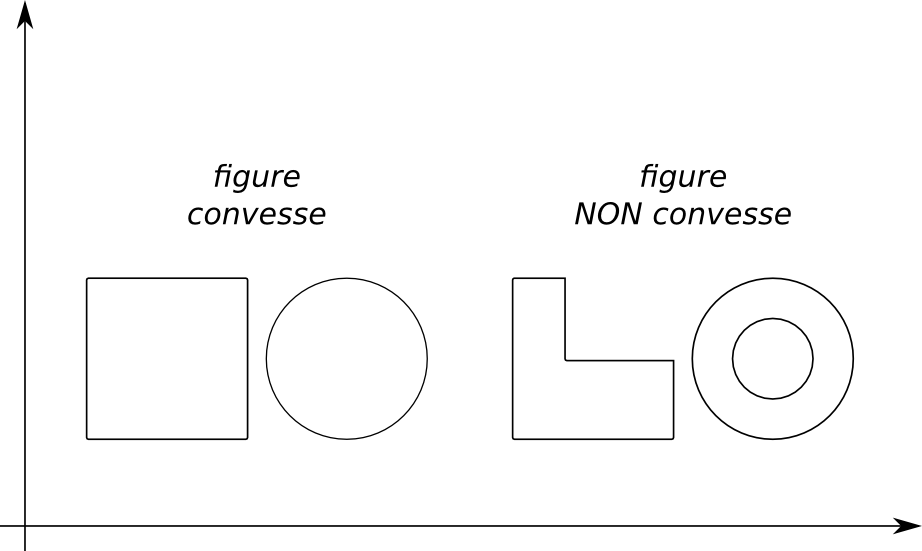
\includegraphics[width=0.5\textwidth]{images/convessita.png}
  \caption{Insiemi convessi e non convessi}
  \label{convessita}
\end{figure}

\par\bigskip

{\bf Propriet\`a}: dati {\em n} insiemi $S_i$ convessi (con {\em i}
che va da 1 a {\em n}), la loro intersezione $I = \cap_{i=1}^n S_i$ \`e un
insieme convesso.\\
{\bf Dimostrazione}: prendiamo due punti $x, y \in I$. Dato che
appartengono all'intersezione, appartengono a tutti gli $S_i$. La
combinazione convessa di $x$ e $y$ appartiene a tutti gli $S_i$ visto
che sono insiemi convessi, quindi appartiene anche ad $I$ che dunque
\`e convesso. $\blacksquare$

\par\bigskip

{\bf Definizione di \underline{funzione convessa}}: una funzione
$c:S\rightarrow \mathbb{R}^1$ si dice convessa in $S$ se vale la
seguente propriet\`a:

\begin{center}
$c(\lambda\cdot x + (1-\lambda)\cdot y) \leq \lambda\cdot c(x) +
  (1-\lambda)\cdot c(y) \quad \forall x, y \in S, \quad \forall \lambda
  : 0 \leq \lambda \leq 1$
\end{center}

\begin{figure}[H]
  \centering
  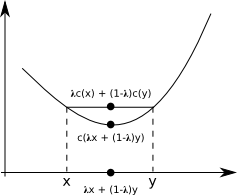
\includegraphics[width=0.33\textwidth]{images/funzioneconvessa.png}
  \caption{Funzione convessa}
  \label{funzioneconvessa}
\end{figure}

\par\bigskip

{\bf Propriet\`a}: data una funzione {\em c} convessa su un insieme {\em S}
convesso ed un valore {\em t}, l'insieme $S_t = \{ x \in S : c(x) \leq
t\}$ \`e convesso.\\
{\bf Dimostrazione}: prendiamo due punti $x,y \in S_T$. La loro
combinazione convessa ovviamente apparterr\`a a {\em S}, dato che sono
due punti di {\em S} prima ancora che di $_t$. Per dimostrare che la
combinazione convessa appartiene a $_t$ scriviamo:

\begin{center}
$c(\lambda\cdot x + (1-\lambda)\cdot y) \leq \lambda\cdot c(x) +
  (1-\lambda)\cdot c(y) \leq \lambda\cdot t +
  (1-\lambda)\cdot t = t$
\end{center}

\noindent da cui si ha $\lambda\cdot x + (1-\lambda)\cdot y \in S_t$.
$\blacksquare$

\begin{figure}[H]
  \centering
  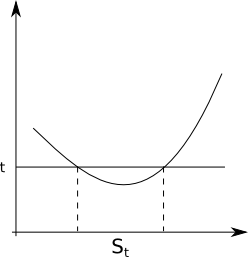
\includegraphics[width=0.33\textwidth]{images/insiemeconvesso.png}
  \caption{Insieme convesso}
  \label{insiemeconvesso}
\end{figure}

\par\bigskip

{\bf Definizione di \underline{funzione concava}}: una funzione $c(x)$
\`e concava se la funzione $-c(x)$ \`e convessa. Una funzione lineare
\`e sia concava che convessa.

\section{Programmazione convessa}

Vediamo cosa si intende con programmazione convessa e quali sono le
principali propriet\`a\dots

\par\bigskip

{\bf Definizione di \underline{programmazione convessa}}: un problema
\`e di programmazione convessa se il suo obiettivo \`e minimizzare una
funzione convessa su un insieme convesso.

\par\bigskip

{\bf Teorema}: dato un problema $(F,c)$ con {\em F} convesso e {\em c}
funzione convessa su {\em F}, l'intorno euclideo $N_\varepsilon(x)$
\`e esatto per qualunque $\varepsilon > 0$.\\
{\bf Dimostrazione}: sia $x$ un ottimo locale rispetto a
$N_\varepsilon$ e consideriamo un punto $y$ esterno a tale
intorno. Una combinazione convessa di $x$ e $y$ \`e data da $z =
\lambda\cdot x + (1-\lambda)\cdot y$ e giace sul segmento che unisce {\em x}
 a {\em y}. \`E tanto pi\`u prossima a {\em x} quanto pi\`u $\lambda$
 \`e prossimo a 1. Scegliendo valori di $\lambda$ tali da prendere
 punti {\em z} appartenenti all'intorno, ed essendo {\em c} convesso,
 svolgiamo i seguenti passaggi:

 \begin{center}
$c(z) \leq \lambda\cdot c(x) + (1-\lambda)\cdot c(y)$
 \end{center}

\noindent da cui:

\begin{center}
$c(y) \geq \frac{c(z)-\lambda c(x)}{1-\lambda}$  
\end{center}

\noindent e considerando che $z \in N_\varepsilon(x)$ (perch\'e {\em x} \`e un
ottimo locale, dunque \`e pi\`u piccolo di ogni altro elemento in
$N_\varepsilon$) si ha:

\begin{center}
$c(y) \geq \frac{c(x)-\lambda c(x)}{1-\lambda} = c(x)$   
\end{center}

\noindent cio\`e $x$ \`e ottimo rispetto ad un qualunque punto $y \in
F$. $\blacksquare$

\par\bigskip

{\bf Teorema}: se la funzione $\varphi$ \`e convessa, le funzioni $g_i$
sono concave $\forall i$ e le $h_j$ sono lineari $\forall j$, allora
il modello di programmazione relativo \`e un problema di
programmazione convessa.\\
{\bf Dimostrazione}: per definizione la funzione $\varphi$ \`e convessa,
dunque ci resta da dimostrare che la regione ammissibile \`e
convessa. Le funzioni lineari $h_j$ le possiamo vedere come l'unione
di due vincoli:

\begin{center}
$h_j(x) \geq 0 \qquad -h_j(x) \geq 0$  
\end{center}

che sono due funzioni concave. Queste, unite alle funzioni $g_i$,
concave anch'esse, definiscono una regione ammissibile del tipo:

\begin{center}
$\{ x \in \mathbb{R}^n : f_l(x) \geq 0 \} = \{ x \in \mathbb{R}^n :
  -f_l(x) \leq 0 \}$
\end{center}

dove ogni $-(f_l(x))$ \`e convessa $\forall l$. Abbiamo quindi
un'intersezione di regioni convesse, dunque un insieme
convesso. $\blacksquare$

%%%%%%%%%%%%%%%%%%%%%%%%%%%%%%%%%%%%%%%%%%%%%%%%%%%%%%%%%%%%%%
%%
%% CAPITOLO 3 - PROGRAMMAZIONE LINEARE
%%
%%%%%%%%%%%%%%%%%%%%%%%%%%%%%%%%%%%%%%%%%%%%%%%%%%%%%%%%%%%%%%

\chapter{Programmazione lineare}

\section{Problemi in due dimensioni}

Quando si ha a che fare con un problema in due dimensioni \`e
possibile risolverlo per via grafica e ci\`o ci consente di capire
meglio il funzionamento di tali problemi.

Sul grafico, per diversi valori di {\em z} possiamo tracciare diverse
rette parallele (normali al gradiente). Noi siamo chiaramente
interessati alla soluzione di valore minimo (se il problema \`e di
minimizzazione), dunque dopo aver disegnato la regione ammissibile, la
retta di interesse \`e quella che tocca l'ultimo pezzo di regione
prima di uscirne nella direzione contraria al gradiente (che si
calcola con $(\partial z / \partial x_1, \partial z / \partial x_2)$).

\section{Forma generale, canonica e standard}

Basandoci sulle notazioni introdotte all'inizio del precedente
capitolo, faremo riferimento da questo momento a problemi in cui {\em
  A} \`e una matrice $m \times n$, {\em b} \`e un vettore intero di
{\em m} elementi e {\em c} \`e un vettore intero di {\em n} elementi.

\par\bigskip

Vediamo ora in quali forme si pu\`o esprimere un problema di {\bf
  programmazione lineare} (LP).

\vspace{20pt}
\begin{center}
  \begin{tabular}{l|l|l}
    {\bf Forma generale} & {\bf Forma canonica} & {\bf Forma standard}
    \\\hline
    $\min c'x$ & $\min c'x$ & $\min c'x$ \\
    $\quad a_i'x = b_i \quad \forall i \in M$ & $\quad Ax \geq b$ &
    $\quad Ax = b$ \\
    $\quad a_i'x \geq b_i \quad \forall i \in \bar{M}$ & $\quad x\geq
    0$ & $\quad x \geq 0$ \\
    $\quad x_j \geq 0 \quad \forall j \in N$ && \\
    $\quad x_j \gtreqless 0 \quad \forall j \in \bar{N}$ && \\
  \end{tabular}
\end{center}
\vspace{20pt}

\section{Esempio: il problema della dieta}

Il {\bf problema della miscelazione} o {\bf problema della dieta} \`e
il classico esempio di problema di programmazione lineare.

\par\bigskip

Un allevatore deve preparare il mangime per i suoi animali e lo deve
fare miscelando {\em n} prodotti con {\em m} sostanze nutritive
diverse. Per ogni sostanza nutritiva {\em j} si conosce il fabbisogno
minimo mensile $b_j$ e di ogni prodotto {\em i} se ne conosce il costo
$c_i$. Ogni elemento $a_{ij}$ della matrice {\em A} indica la
quantit\`a di sostanza $j$ contenuta nel prodotto $i$.

Il problema consiste nel determinare il valore di ogni variabile $x_j$
dove $x_j$ \`e la quantit\`a di prodotto $j$ da acquistare mensilmente.

\section{Basi e soluzioni base}

{\bf Definizione di \underline{base}}: chiamiamo {\bf base} della
matrice {\em A} l'insieme di {\em m} colonne linearmente indipendenti
(assumiamo, ma lo vedremo nella prossima sezione che la matrice {\em
  A} sia di rango {\em m}). Indicando con $\beta(i)$ ($i = 1,\dots,m$)
gli indici di tali colonne, possiamo dire che la base \`e:
$\mathcal{B} = \{A_{\beta(1)},\dots,A_{\beta(m)}\}$. Una base
$\mathcal{B}$ individua una sottomatrice quadrata $m\times m$ che
indichiamo con $B = [A_{\beta(i)}]$.

\par\bigskip

{\bf Definizione di \underline{soluzione base}}: chiamiamo soluzione
di base corrispondente alla base $\mathcal{B}$, la soluzione che si
ottiene sfruttando gli $n-m$ gradi di libert\`a del problema per
porre a 0 le variabili fuori base e risolvere il problema $Bx_{\beta}
= b$ risultante.

\par\bigskip

{\bf Definizione di \underline{soluzione di base ammissibile}}: non
tutte le soluzioni di base sono ammissibili. Se oltre a risolvere il
sistema $Bx_\beta = b$ rispettano anche il vincolo $x\geq 0$, allora
la soluzione \`e detta soluzione di base ammissibile (SBA).

\section{Assunzioni per il metodo del simplesso}

Per introdurre l'algoritmo del simplesso faremo quattro assunzioni:

\begin{itemize}
\item {\bf Assunzione 0}: i problemi presi in considerazione sono in
  forma standard con $m < n$.

\item {\bf Assunzione 1}: la matrice {\em A} possiede {\em m} colonne
  linearmente indipendenti, ossia \`e di rango {\em m}.

\item {\bf Assunzione 2}: la regione ammissibile non \`e vuota.

\item {\bf Assunzione 3}: la regione ammissibile \`e limitata nella
  direzione di decrescita del gradiente.
\end{itemize}

Mentre l'assunzione 0 non fa perdere di generalit\`a l'algoritmo, le
assunzioni 1, 2 e 3 dovranno essere verificate dall'algoritmo. Nel
caso in cui queste assunzioni siano violate, l'algoritmo dovr\`a
comunque essere in grado di trovare la soluzione ottima.

\par\bigskip

A questo punto dimostriamo per quale motivo l'assunzione 0 non fa
perdere di generalit\`a all'algoritmo. Dobbiamo dimostrare che le tre
forme (generale, canonica e standard) sono equivalenti e che i casi in
cui $m=n$ e $m>n$ non risultano interessanti. Iniziamo proprio da
questo.

\par\bigskip

Per il {\bf teorema di Rouche-Capelli} i problemi in cui $m > n$ non
hanno soluzione. I problemi in cui $m=n$ prevedono una sola soluzione,
dunque non ha senso parlare di problemi di ottimizzazione. Infine nel
caso in cui $m < n$ abbiamo $n-m$ gradi di libert\`a e $\infty^{n-m}$
soluzioni. In questo caso dunque ha senso parlare di problemi di
ottimizzazione in quanto siamo interessati a trovare la soluzione
ottima fra infinite soluzioni. 

\par\bigskip

Ora vediamo come le tre forme siano equivalenti. Le seguenti regole ci
permettono di passare da una forma all'altra:

\begin{itemize}

\item un vincolo nella forma $x_j \gtreqless 0$ pu\`o essere sostituito
con $x_j = x_j^+ + x_j^-$ con $x_j^+ \geq 0$ e $x_j^- \geq 0$;

\item un vincolo $a_i'x = b_i$ \`e equivalente alla coppia di vincoli
  $a_i'x \geq b_i$, $a_i'x \leq b_i$;

\item un vincolo $a_i'x \geq b_i$ \`e equivalente al vincolo $a_i'x -
  s_i = b_i$, dove $s_i$ prende il nome di {\bf variabile surplus};
  
\item un vincolo $a_i'x \leq b_i$ \`e equivalente al vincolo $a_i'x +
  s_i = b_i$, dove la variabile $s_i$ prende il nome di {\bf variabile
  slack}.

\end{itemize}

\section{Politopi convessi}

{\bf Definizione di \underline{iperpiano}}: dato uno spazio
$\mathcal{R}^d$ di dimensione {\em d}, dato un vettore $h \neq 0$
di {\em d} elementi e dato uno scalare {\em g}, definiamo {\bf
  iperpiano} l'insieme dei punti $\{ x : h'x = g \}$. L'iperpiano
divide lo spazio in due {\bf semispazi} $\{x : h'x \leq g\}$ e $\{x :
h'x \geq g\}$.

%% TODO: figura

\par\bigskip

{\bf Definizione di \underline{politopo}}: l'intersezione di un numero
finito di semispazi \`e detta {\bf politopo}. Spesso, ma non tutti gli
autori concordano, si richiede che l'intersezione sia limitata e non
vuota.

\par\bigskip

{\bf Definizione di \underline{dimensione di un politopo}}: la
dimensione di un politopo \`e la dimensione del pi\`u piccolo spazio
in grado di contenerlo. 

\par\bigskip

{\bf Propriet\`a}: la regione ammissibile di un problema di
programmazione lineare \`e un politopo.\\ {\bf Dimostrazione}: basta
considerare che un problema di programmazione lineare pu\`o sempre
essere posto in forma canonica, di conseguenza la regione ammissibile
pu\`o essere definita dall'intersezione di un insieme finito di
semispazi. $\blacksquare$

\par\bigskip

{\bf Definizione di \underline{faccia}}: dato un politopo {\em P} ed
un iperpiano {\em H} non necessariamente legato a {\em P} e sia {\em
  HS} uno dei due semispazi definiti da {\em H}. Chiamiamo {\em
  faccia} del politopo l'insieme $f = P \cap HS$ se rispetta le due
condizioni:

\begin{center}
$f \subset H \quad$ e $\quad f \neq \emptyset$
\end{center}

\par\bigskip

{\bf Definizione di \underline{faccetta}}: chiamiamo {\bf faccetta}
una faccia di dimensione $d-1$ (dove {\em d} \`e la dimensione del
politopo).

\par\bigskip

{\bf Definizione di \underline{spigolo}}: uno {\bf spigolo} \`e un
vertice di dimensione 1.

\par\bigskip

{\bf Definizione di \underline{vertice}}: un {\bf vertice} \`e una
faccia di dimensione 0.

\par\bigskip

{\bf Definizione di \underline{combinazione convessa di {\em p}
    punti}}: estendiamo il concetto di combinazione convessa a {\em p}
punti $x^{(1)},\dots,x^{(p)} \in \mathbb{R}^n$. Tale combinazione
convessa \`e data da:

\begin{center}
$\sum\limits_{i=1}^p \alpha_i x^i \qquad \biggr(\sum\limits_{i=1}^p \alpha_i
  = 1, \quad \alpha_i \geq 0 \forall i\biggr)$  
\end{center}

\par\bigskip

{\bf Teorema}: ogni punto $p \in P$ \`e combinazione convessa dei
vertici del politopo. Ogni combinazione convessa dei vertici \`e un
punto del politopo.

\par\bigskip

{\bf Teorema}: un vertice non \`e combinazione convessa stretta di due
punti distinti del politopo (cio\`e la combinazione convessa
dev'essere $0\leq\lambda\leq1$ e non $0 < \lambda < 1$).\\
{\bf Dimostrazione}: ci limitiamo a dimostrare la sufficienza e lo
facciamo {\bf per assurdo}. Prendiamo un vertice $v \in P$ e
supponiamo che esistano due vertici $w,y \in P$ tali che:

\begin{center}
$v = \lambda\cdot y + (1-\lambda)\cdot w$  
\end{center}

Dal momento che $v$ \`e un vertice, cio\`e una faccia di dimensione 0,
dovr\`a esistere un semispazio $HS$ tale che $P \cap HS = \{ v
\}$. Questo semispazio possiamo supporre che sia $\{x : h'x \geq g
\}$. Dato che l'intersezione di $HS$ con $P$ contiene solo $v$, non
pu\`o contenere anche $y$ e $w$, quindi questi due elementi non
possono essere contenuti nel semispazio e devono perci\`o valere $h'y <
g$ e $h'w < g$. Segue dunque:

\begin{center}
$h'v = h'(\lambda\cdot y + (1-\lambda)\cdot w) = \lambda\cdot y +
  (1-\lambda)\cdot w > g$  
\end{center}

il che ci dice che $v \not\in HS$ che \`e assurdo. $\blacksquare$

\section{Relazione fra politopi e soluzioni base}

{\bf Propriet\`a}: l'insieme dei vincoli di un LP definisce un
politopo. \small({\em in realt\`a tale propriet\`a \`e stata gi\`a
  citata e dimostrata in precedenza\dots})\normalsize\\
{\bf Dimostrazione}: \`e sufficiente dimostrare che ogni problema
pu\`o essere portato in forma canonica e i vinoli di un problema in
forma canonica definiscono un'intersezione di semispazi non vuota (per
l'assunzione 2) e limitata (per la 3).$\blacksquare$

\par\bigskip

{\bf Teorema}: dato un politopo {\em P} definito dai vincoli di un LP,
condizione necessaria e sufficiente affinch\'e un punto sia un vertice
\`e che il corrispondente vettore {\em x} sia una SBA.\\ {\bf
  Dimostrazione}: dimostriamo prima la {\bf sufficienza}. Prendiamo
una SBA $x_\beta = (x_{\beta(1)},\dots,x_{\beta(m)})$ a cui
corrisponde ovviamente l'inseme di colonne $\mathcal{B} = \{
A_{\beta(1)},\dots,A_{\beta(m)}\}$. Essendo una SBA soddisfa il
sistema $Ax = b$, quindi possiamo scrivere:

\begin{center}
$\sum\limits_{A_j \in \mathcal{B}} x_j = b$  
\end{center}

A questo punto dobbiamo dimostrare che tale SBA \`e un vertice. Se \`e
un vertice non \`e combinazione convessa stretta di due punti distinti
$y, w\in P$. Supponiamo dunque per assurdo che lo sia, dunque che
valga:

\begin{center}
$x = \lambda \cdot y + (1-\lambda) \cdot w \quad (0 < \lambda < 1)$ 
\end{center}

Poich\'e dobbiamo avere $x \geq 0$, dobbiamo anche essere certi che $w
\geq 0$ e $y \geq 0$ e che lo siano per ogni componente, dunque $w_j, y_j
\geq 0 \forall j$. $x$ \`e inoltre nullo per le componenti fuori base
e altrettanto dobbiamo richiedere a $w$ e $y$. Conseguono dunque le
due relazioni:

\begin{center}
$\sum\limits_{A_j \in \mathcal{B}} y_jA_j =b \qquad \sum\limits_{A_j
    \in \mathcal{B}} w_jA_j =b$
\end{center}

da cui, sottraendo alla prima relazione scritta:

\begin{center}
$\sum\limits_{A_j \in \mathcal{B}} (x_j-y_j)A_j = 0 \qquad \sum\limits_{A_j
    \in \mathcal{B}} (x_j-w_j)A_j = 0$
\end{center}

Dal momento che le colonne $A_j$ sono linearmente indipendenti,
l'unico modo per avere 0 \`e che i coefficienti $(x_j-w_j)$ e
$(x_j-y_j)$ siano 0, dunque avremmo $x \equiv w \equiv y$ e ci\`o {\bf
  contraddice} l'ipotesi di combinazione convessa stretta.

\par\bigskip

Dimostriamo ora la {\bf necessit\`a} che {\em x} sia una SBA
affinch\'e sia un vertice. Dato un vertice $x$ del politopo, definiamo
l'insieme delle colonne di {\em A} a cui corrisponde un $x_j$
strettamente positivo: $\mathcal{C} = \{ A_j : x_j > 0\}$. Queste
colonne sono sicuramente in base, altrimenti avrebbero il
corrispondente $x_j$ pari a 0. Essendo in base sono linearmente
indipendenti. Supponiamo per assurdo che non lo siano. Se non lo sono,
per avere $\sum\limits_{A_j \in \mathcal{C}} d_jA_j = 0$, devono
esistere $|\mathcal{C}|$ coefficienti $d_j$ non tutti
nulli. Ricordiamo inoltre che $x \in F$, dunque dev'essere maggiore/uguale a
0 in ogni sua componente e deve valere $\sum\limits_{A_j \in
  \mathcal{C}}x_jA_j = b$. Facciamo la somma o la differenza fra queste ultime
due relazioni ed otteniamo:

\begin{center}
$\sum\limits_{A_j \in \mathcal{C}} (x_j+\vartheta d_j)A_j = b \qquad
  \sum\limits_{A_j \in \mathcal{C}} (x_j-\vartheta d_j)A_j = b$
\end{center}

dove $\vartheta$ \`e uno scalare sufficientemente piccolo da garantire
che il coefficiente di $A_j$ sia maggiore uguale a 0. Con questo
procedimento abbiamo ottenuto due punti di {\em F} che hanno come
coordinate:

\begin{center}
\[\left\{
  \begin{array}{l l}
    x_j^{(1)} = x_j + \vartheta d_j, x_j^{(2)} = x_j - \vartheta d_j &
    \quad \text{se $A_j \in \mathcal{C}$}\\
    x_j^{(1)} = x_j^{(2)} = 0& \quad \text{se $A_j \not\in\mathcal{C}$}\\
  \end{array} \right.\]
\end{center}

Otteniamo $x = \frac{1}{2}x^{(1)} + \frac{1}{2}x^{(2)}$, dunque $x$
\`e combinazione convessa stretta di due punti del politopo, dunque
non \`e un vertice: {\bf assurdo}.

Abbiamo dunque che le colonne $A_j \in \mathcal{C}$ sono linearmente
indipendenti e deve aversi $|\mathcal{C}|\leq m$. Se \`e minore di
{\em m}, possiamo aggiungere $m-|\mathcal{C}|$ colonne per ottenere un
insieme di colonne linearmente indipendenti cui corrisponde lo stesso
{\em x}. A {\em x} corrisponde un insieme di colonne linearmente
indipendenti, cio\`e una SBA. $\blacksquare$

\par\bigskip

{\bf Teorema}: dato un qualunque problema LP, esiste sempre un vertice
ottimo (cio\`e esiste sempre una SBA ottima).\\ {\bf Dimostrazione}:
consideriamo un problema LP definito da $\min{c'x}$, dove $c$ \`e il
vettore costo. Sia {\em P} il politopo della regione ammissibile
delimitato dai vertici $x^{(1)},\dots,x^{(p)}$. Sia $x^{(0)}$ il
vertice corrispondente alla soluzione ottima. Essendo un vertice si
pu\`o esprimere come combinazione convessa degli altri vertici,
dunque:

\begin{center}
$x^{(0)} = \sum_{i=1}^{p} \alpha_i x^{(i)}\qquad \biggr (
  \sum\limits_{i=1}^p \alpha_i = 1, \alpha_i
  \geq0 \forall i \biggr )$  
\end{center}

Ora sia $x^{(j)}$ il vertice di costo minimo, cio\`e tale per cui
$c'x^{(j)} = \min\limits_{1\leq i\leq p}\{
c'x^{(i)}\}$. Moltiplichiamo per $c$ la prima relazione
espressa e relazioniamola con $x^{(j)}$. Varr\`a allora:

\begin{center}
$c'x^{(0)} = c'\sum\limits_{i=1}^p \alpha_i x^{(i)} \geq
  c'\sum\limits_{i=1}^p \alpha_i x^{(j)} =
  c'x^{(j)}\sum\limits_{i=1}^p \alpha_i = c'x^{(j)}$  
\end{center}

Dal momento per\`o che \underline{non} pu\`o essere $c'x^{(j)} >
c'x^{(0)}$, deve aversi $c'x^{(j)} = c'x^{(0)}$. Bisogna fare
attenzione per\`o che in questo modo non abbiamo dimostrato che il
vertice di costo minimo coincida con il punto ottimo, ma che ha lo
stesso costo. $\blacksquare$

\par\bigskip

{\bf Teorema}: ogni combinazione convessa di vertici ottimi \`e
ottima.\\
{\bf Dimostrazione}: siano $x^{(1)},\dots,x^{(q)}$ dei vertici ottimi
e consideriamo una loro combinazione convessa:

\begin{center}
$x = \sum\limits_{i=1}^q \alpha_i x^{(i)} \qquad \biggr (
  \sum\limits_{i=1}^q \alpha_i = 1, \alpha_i \geq 0 \forall i \biggr
  )$
\end{center}

Moltiplichiamo per il vettore costo {\em c}:

\begin{center}
$c'x = c' \sum\limits_{i=1}^q \alpha_i x^{(i)} = c'x^{(1)}
  \sum\limits_{i=1}^q \alpha_i = c'x^{(1)}$. $\blacksquare$
\end{center}

\section{Basi degeneri}

Due SBA diverse sono prodotte sicuramente da due basi diverse, ma due
basi diverse \underline{non} \`e detto che producano la stessa SBA.

\par\bigskip

{\bf Definizione di \underline{base degenere}}: una SBA che possiede
pi\`u di $n-m$ zeri si dice {\bf degenere}.

\par\bigskip

{\bf Propriet\`a}: se due basi producono la stessa SBA {\em x}, allora
{\em x} si dice {\bf degenere}.\\ {\bf Dimostrazione}: se prendiamo
due basi $\mathcal{B}$ e $\bar{\mathcal{B}}$ che producono la stessa
SBA noteremo che la SBA prodotta da $\mathcal{B}$ contiene $n-m$ zeri
in corrispondenza delle variabili non in base pi\`u uno zero in ogni
colonna dell'insieme
$\mathcal{B}\textbackslash\bar{\mathcal{B}}$. $\blacksquare$

\chapter{TODO Algoritmo del simplesso}
\chapter{TODO Dualit\`a}

%%%%%%%%%%%%%%%%%%%%%%%%%%%%%%%%%%%%%%%%%%%%%%%%%%%%%%%%%%%%%%
%%
%% CAPITOLO 6 - Programmazione lineare intera
%%
%%%%%%%%%%%%%%%%%%%%%%%%%%%%%%%%%%%%%%%%%%%%%%%%%%%%%%%%%%%%%%

\chapter{Programmazione lineare intera}

I problemi di {\bf programmazione lineare intera} (PLI) hanno la
caratteristica di imporre un vincolo di interezza sulle
variabili. Abbiamo dunque un modello (in forma standard) come quello
che segue:

\begin{center}
  
  \begin{tabular}{l}
    $\min c'x$ \\
    $\quad Ax = b$ \\
    $\quad x \geq 0, intere$
  \end{tabular}

\end{center}

Eliminando il vincolo di interezza si ottiene il cosiddetto {\bf
  rilassamento continuo} del problema, che altro non \`e che la
versione PL del problema. 

\par\bigskip

{\bf Propriet\`a}: un'importante propriet\`a che lega la soluzione del
problema di PLI a quella del suo rilassamento \`e la seguente:

\begin{center}
$Z(PL) \leq Z(PLI)$  
\end{center}

ovvero la soluzione del rilassamento \`e sempre minore uguale (e
quindi \underline{migliore}) di quella del problema originario.\\
{\bf Dimostrazione}: \`e sufficiente considerare che la regione
ammissibile del problema di PL contiene quella del problema di PLI
(che \`e composta soltanto dai punti interi contenuti al suo
interno). $\blacksquare$

\par\bigskip

Se il rilassamento \`e impossibile \`e impossibile anche il problema
di PLI, inoltre se \`e illimitato il primo \`e illimitato anche il
secondo.  Nel caso in cui la soluzione ottima del rilassamento
continuo sia intera, questa corrisponde alla soluzione ottima del
problema di PLI. A questo punto potremmo pensare di trovare la
soluzione ottima semplicemente risolvendo il rilassamento continuo e,
nel caso in cui la soluzione non sia intera, potremmo risolvere
arrotondandola al pi\`u vicino intero. Sbagliato! Non possiamo farlo
perch\'e non avremmo garanzie che la soluzione trovata con
arrotondamento sia davvero ammissibile, n\`e che sia quella ottima per
il problema di PLI.

\section{Unimodularit\`a}

{\bf Definizione di \underline{matrice unimodulare}}: una matrice {\em
  B} quadrata e intera ($m \times m$) si dice {\bf unimodulare} (UM)
se $\det{B} = \pm 1$.

\par\bigskip

{\bf Definizione di \underline{matrice totalmente unimodulare}}: una
matrice {\em A} rettangolare intera ($m \times n$) si dice {\bf
  totalmente unimodulare} (TUM) se ogni sua sottomatrice quadrata non
singolare {\em B} \`e unimodulare.

\par\bigskip

{\bf Teorema}: se una matrice {\em A} \`e TUM, allora i vertici della
regione ammissibile $\{ x : Ax = b, x \geq 0 \}$ sono interi $\forall
b$ intero.\\
{\bf Dimostrazione}: prendiamo la sottomatrice {\em B} corrispondente
ad una base. La soluzione base pu\`o essere scritta come:

\begin{center}
$x = B^{-1}b = \frac{B^a}{\det{B}}\cdot b$  
\end{center}

ed essendo {\em B} unimodulare (visto che {\em A} \`e TUM), allora la
soluzione {\em x} \`e intera. $\blacksquare$

\par\bigskip

Il risultato che abbiamo appena indicato, come possiamo notare, vale
per regioni ammissibili di problemi in forma standard. L'estensione a
problemi in forma generale/canonica \`e data dal prossimo teorema.

\par\bigskip

{\bf Teorema}: se una matrice {\em A} \`e TUM, allora i vertici della
regione ammissibile $\{x : Ax \leq 0, x \geq 0 \}$ sono interi
$\forall b$ intero.\\
{\bf Dimostrazione}: dal momento che il problema non \`e in forma
standard, lo riconduciamo a quello in modo da poter sfruttare il
precedente teorema. Per portarlo in forma standard dobbiamo aggiungere
delle variabili di slack che ci portano ad avere la matrice
$(A|I)$. Dobbiamo quindi dimostrare che $(A|I)$ sia TUM. Prendiamo
perci\`o tutte le sottomatrici e vediamo se sono UM. Sicuramente
prendendo delle sottomatrici solo di A o solo di I il risultato \`e un
minore unimodulare. Ci\`o che dobbiamo ancora discutere \`e invece
l'unimodularit\`a di sottomatrici prese {\em sul confine} fra {\em A}
e {\em I}. Chiamiamo {\em C} una tale matrice. Tramite permutazioni
delle righe la riconduciamo alla forma:

\begin{center}
$\tilde{C} = \biggr (
 \begin{array}{c|c}
  B & 0 \\
  \hline
  D & I
 \end{array}
\biggr )$
\end{center}

Il determinante di $\tilde{C}$ \`e uguale a quello di {\em B}, da cui
$\det{C} = \pm \det{\tilde{C}} = \pm 1$. $\blacksquare$

\par\bigskip

Ricapitolando, se una matrice \`e TUM i vertici della regione
ammissibile (su cui si troveranno le soluzioni) sono interi! Per
problemi dove {\em A} \`e TUM basta dunque risolvere il rilassamento
continuo. Per matrici non TUM bisogner\`a introdurre altre metodologie
(algoritmi {\em branch and bound} o algoritmi basati sui piani di
taglio).

\section{Algoritmi cutting-plane}

Gli algoritmi dei piani di taglio permettono di risolvere problemi di
PLI tagliando porzioni della regione ammissibile dopo che si \`e
trovata una soluzione $x^*$ non intera. Tali porzioni:

\begin{itemize}
\item {\bf \underline{non}} devono per\`o eliminare alcuna soluzione
  ammissibile;
\item devono eliminare dalla regione ammissibile la zona contenente
  $x^*$.
\end{itemize}

\subsection{Tagli di Gomory}

Il metodo dei tagli di Gomory \`e stato il primo algoritmo cutting
plane sviluppato ed \`e ancora oggi molto utilizzato. Vediamo dunque
come genera i tagli, ma introduciamo prima una nozione che ci sar\`a
utile.

\par\bigskip

{\bf Definizione di \underline{parte intera}}: dato un numero $y \in
\mathbb{R}^1$, chiamiamo parte intera di {\em y} e la indichiamo con
$\lfloor y \rfloor$ il massimo intero {\em q} tale che $q \leq y$.

\par\bigskip

Sia $\mathcal{B}$ una base ottima del problema, cui corrisponde la SBA
ottima $(x_{\beta(1)}, x_{\beta(2)}, \dots, x_{\beta{m}})$. Possiamo
scrivere per ogni $i$, la seguente relazione:

\begin{center}
$x_{\beta(i)} + \sum\limits_{A_j \not\in \mathcal{B}} y_{ij}x_j = y_{i0}$  
\end{center}

Dato che consideriamo valori di $x$ maggiori o uguali a 0, possiamo
dire che vale la relazione:

\begin{center}
$\sum\limits_{A_j \not\in \mathcal{B}} \lfloor y_{ij} \rfloor x_j \leq
  \sum\limits_{A_j \not\in \mathcal{B}} y_{ij}x_j$
\end{center}

Se sostituiamo nella prima equazione otteniamo:

\begin{center}
$x_{\beta(i)} + \sum\limits_{A_j \not\in \mathcal{B}} \lfloor y_{ij}
  \rfloor x_j \leq y_{i0}$  
\end{center}

e considerando che $x$ dev'essere intero possiamo ulteriormente
trasformarla in: 

\begin{center}
$x_{\beta(i)} + \sum\limits_{A_j \not\in \mathcal{B}} \lfloor y_{ij}
  \rfloor x_j \leq \lfloor y_{i0}\rfloor$  
\end{center}

Facendo la differenza fra la prima equazione e quest'ultima relazione
abbiamo:

\begin{center}
$\sum\limits_{A_j \not\in \mathcal{B}} (y_{ij} - \lfloor y_{ij}
  \rfloor) x_j \geq (y_{i0} - \lfloor y_{i0} \rfloor)$  
\end{center}

Se chiamiamo {\bf parte frazionaria} la differenza fra una variabile e
la sua parte intera $y_{ij} - \lfloor y_{ij} \rfloor$ e la indichiamo
con $f_{ij}$, possiamo riscrivere la relazione come:

\begin{center}
$\sum\limits_{A_j \not\in \mathcal{B}} f_{ij} x_j \geq f_{i0}$  
\end{center}

\`E da questa relazione che otteniamo il taglio. Dobbiamo portarla in
forma standard, dunque moltiplichiamo per $-1$ ed aggiungiamo una
variabile di slack {\em s}. Il {\bf taglio di Gomory} \`e dunque:

\begin{center}
$-\sum\limits_{A_j \not\in \mathcal{B}} f_{ij} x_j + s = -f_{i0}$  
\end{center}

Dobbiamo per\`o ancora dimostrare che tale soluzione \`e ci\`o che fa
per noi\dots

\par\bigskip

{\bf Teorema}: Se aggiungiamo al tableau finale il taglio
$-\sum\limits_{A_j \not\in \mathcal{B}} f_{ij} x_j + s = -f_{i0}$:

\begin{enumerate}
\item non si elimina alcun punto intero ammissibile;
\item il nuovo tableau contiene una base non ammissibile per il
  primale (se $y_{i0}$ \underline{non} \`e intero) ed ammissibile per
  il duale.
\end{enumerate}
{\bf Dimostrazione}: possiamo osservare che abbiamo operato imponendo
unicamente condizioni di interezza, dunque il primo punto \`e
dimostrato. Per quanto riguarda il punto {\em 2}, notiamo che se
$y_{i0}$ \underline{non} \`e intero otteniamo un valore negativo in
colonna 0, dunque la soluzione non \`e pi\`u ammissibile per il
problema primale. In riga 0 in corrispondenza della nuova variabile in
base {\em s} poniamo 0 perci\`o il criterio di ottimalit\`a \`e ancora
soddisfatto, dunque ci sono i presupposti per l'applicazione del
simplesso duale. $\blacksquare$

\section{Branch and bound}

Gli algoritmi branch and bound sono una metodologia introdotta nel
1960 ed utilizzabile per qualunque problema avente struttura
combinatoria. Come possiamo immaginare avremo due fasi, una di {\bf
  branching} ed una di {\bf bounding}.

\subsection{Branching}

Si generano da un problema $P$ dei sottoproblemi $P^k$ (con
$k=1,2,\dots$). Per ogni problema $P^k$ si indica con $x^k$ la
soluzione ottima del suo rilassamento continuo, mentre con $z^k$ il
valore della soluzione ottima.

\par\bigskip

Supponendo di aver trovato una soluzione in cui la variabile $x_i$ ha
un valore $a$ frazionario, generiamo due sottoproblemi, uno dato
dall'aggiunta del vincolo $x_i \leq \lfloor a \rfloor a$ e l'altro
dato dall'aggiunta del vincolo $x_i \geq \lfloor a \rfloor + 1$. Le
due condizioni sono {\bf mutuamente esclusive} nonch\'e {\bf
  esaustive}. I due problemi $P^1$ e $P^2$ generati dovranno
ovviamente essere risolti separatamente. 

\par\bigskip

Ogni problema $P^k$ pu\`o essere ramificato originando due problemi, a
meno che:

\begin{itemize}
\item $x^k$ sia intero;
\item il rilassamento continuo di $P^k$ sia impossibile
\end{itemize}

in quanto in questi casi il problema $P^k$ \`e {\bf risolto}.

\par\bigskip

Come possiamo immaginare, dalla ramificazione dei vari problemi esce
fuori un {\bf albero decisionale}. A $P^0$ corrisponder\`a il {\bf
  nodo padre}. Ad eccezione del nodo padre, ogni nodo presenta un ramo
entrante. Ogni nodo, ad eccezione delle {\bf foglie} presentano due
rami discendenti. Solitamente nella rappresentazione si inserisce,
all'interno dei nodi dell'albero l'ordine con il quale sono stati
esplorati i problemi. A fianco ai nodi si scrive il valore del
rilassamento continuo, mentre a fianco ai rami si scrive la condizione
imposta per generare il sotto problema di destinazione.

\subsection{Bounding}

Gli algoritmi branch and bound non sarebbero cos\`i potenti se si
fermassero al solo branching. A renderli potenti c'\`e il bounding che
consiste nel tagliare dei sottoproblemi le cui soluzioni sicuramente
non sarebbero ottime.

\par\bigskip

Se {\em z} \`e il valore della miglior soluzione intera trovata finora
e per un problema $P^k$ si ha $\lceil L_k \rfloor \geq z$, allora non
occorre risolvere il problema $P^k$. Si dice che tale nodo viene {\bf
  ucciso}.

\subsection{Inserimento dei vincoli nel tableau}

Volendo imporre la condizione $x_i \leq \lfloor a \rfloor$, questa va
portata in forma standard, dunque si aggiunge una variabile di slack e
si ottiene $x_i + s = \lfloor a \rfloor$. Anche nel caso del vincolo
$x_i \geq \lfloor a \rfloor + 1$ si deve portare il vincolo in forma
standard, quindi si moltiplica per $-1$ e si somma la variabile di
slack ottenendo $-x_i + s = -\lfloor a \rfloor - 1 = t$.

\par\bigskip

A questo punto, dopo aver inserito i vincoli nei rispettivi tableau,
si nota che una colonna della base presenta un valore non nullo dove
invece dovrebbe avere 0 e questo \`e dovuto proprio all'inserimento
dei nuovi vincoli. Per risolvere ci\`o si sottrae alla riga inserita,
la riga di $x_i$. Fatto ci\`o \`e necessario proseguire con il {\bf
  simplesso duale}.

\section{Strategie di esplorazione}

\begin{itemize}

\item {\bf Depth-first}: la strategia depth-first opera secondo due
  fasi:

  \begin{itemize}
  \item {\bf forward step}: si genera un figlio dell'ultimo nodo $P^k$
    generato finch\'e si ottiene un problema facilmente risolubile ed
    eventualmente si aggiorna {\em z}, oppure finch\'e non si trova
    $L(P^k) \geq z$ oppure fino a che $P^k$ non si finiscono i figli
    ammissibili non ancora esplorati.

  \item {\bf backward step}: si risale al padre di $P^k$ (che
    chiamiamo $P^p$) e se $L(P^p)<z$ si genera il figlio successivo,
    altrimenti si risale al padre di $P^p$.
  \end{itemize}

  Si termina quando si cerca di risalire al di sopra di $P^0$. Questo
  metodo ha il vantaggio di riuscire a trovare la soluzione abbastanza
  presto e di richiedere strutture dati molto semplici, nonch\'e di
  mantenere pochi nodi aperti per volta. La strategia produce
  rapidamente delle soluzioni ammissibili, il che fa si che aumentino
  le possibilit\`a di uccidere nodi.

\item {\bf Lowest-first}: con questa strategia si esplorano sempre per
  primi i nodi con pi\`u basso lower bound (pi\`u alto se il problema
  \`e di massimizzazione). Questa strategia calcola $L(P^0)$ e
  definisce l'insieme dei nodi attivi $\Pi := \{P^0\}$. Ad ogni
  iterazione si seleziona e rimuove da $\Pi$ il nodo con pi\`u basso
  lower bound, si generano tutti i suoi figli e se ne calcola il
  bound. Se ci sono nodi facilmente risolubili si risolvono ed
  eventualmente si aggiorna {\em z}. Per i nodi non risolubili, questi
  si aggiungono a $\Pi$ soltanto se $L(P^k) \geq z$. L'algoritmo
  termina quando l'insieme $\Pi$ \`e vuoto o quando contiene solo nodi
  per cui $L(P^k) \geq z$.

  La strategia lowest-first ha il vantaggio di trovare la soluzione
  ottima rapidamente perch\'e esplora sempre i nodi pi\`u promettenti
  per primi, tuttavia mantiene un altissimo numero di nodi aperti e
  richiede strutture dati notevolmente complesse. Le soluzioni
  ammissibili non vengono generate rapidamente e questo implica che
  non si possono sfruttare i tagli.

\item {\bf Depth-first rivisitata}: questa strategia effettua un mix
  della depth-first e della lowest first. Opera come una depth-first,
  ma nel forward step genera tutti i figli del noto attuale,
  calcolando i lower bound relativi ed esplorando il figlio per i
  quali questo valore \`e minimo. Nel backtracking si prosegue
  l'esplorazione con il figlio residuo con minimo lower bound.

\item {\bf Breadth-first}: questa strategia esplora in larghezza
  l'albero decisionale. Viene utilizzata raramente. La breadth-first
  genera tutti i figli di $P^0$ e genera di ogni figlio tutti figli
  non facilmente risolubili e cosi via.

\end{itemize}

\section{Altri problemi di ottimizzazione}

Il problema pi\`u generale di tutti \`e il {\bf Mixed Integer Linear
  Programming} (MILP) che contiene sia variabili per le quali si
richiede il vincolo di interezza, sia variabili per le quali \`e
richiesto solo di essere positive. Il modello lo vediamo qui di
seguito:

\begin{center}
\begin{tabular}{l}
$\min{c'x}$ \\
$\quad Ax = b$ \\
$\quad x_j \geq 0 \quad j\in N$\\
$\quad x_j = 0 \quad j\in \bar{N}$
\end{tabular}
\end{center}

I problemi di LP e ILP sono due specializzazioni di questo problema:
nella prima abbiamo solo variabili appartenenti a $N$, nella seconda
solo variabili di $\bar{N}$. Un caso particolare di ILP \`e invece il
problema LP01, in cui le variabili oltre ad essere intere e positive
sono anche vincolate ad assumere valore 0 o 1. Un problema di questo
tipo ha un modello come quello che segue:

\begin{center}
\begin{tabular}{l}
$\min{c'x}$ \\
$\quad Ax = b$ \\
$\quad x_j \in \{ 0,1\}$\\
\end{tabular}
\end{center}

Il caso pi\`u semplice \`e quello in cui la matrice {\em A} \`e
composta da una sola riga e prende il nome di {\bf Problema Knapsack
  0-1} (KP01).

\section{Problema KP01}

Vediamo in dettaglio come applicare un algoritmo branch and bound
prendendo in esame un generico problema KP01. In questi problemi
conviene ordinare gli elementi secondo valori non crescenti del
rapporto fra profitto e peso, per cui assumeremo:

\begin{center}
$\frac{p_1}{w_1} \geq \frac{p_2}{w_2} \geq \dots \geq \frac{p_n}{w_n}$  
\end{center}

Adottiamo un albero decisionale binario in cui ad ogni livello {\em k}
($k = 1, \dots, n$) decidiamo se porre (1) o meno (0) la variabile
$x_k$ in soluzione. Adottiamo inoltre una strategia depth-first in cui
generiamo al primo livello i due nodi $x_1=1$ e $x_1 = 0$. Ad ogni
iterazione, se esiste un nodo attivo generato da $x_j=1$ si ramifica
da questo, altrimenti dall'altro ($x_j = 0$).

\par\bigskip

Ad ogni nodo bisogna calcolare l'{\bf upper bound}. Ricordiamo che
l'upper bound verrebbe di solito calcolato risolvendo il rilassamento
continuo, in questo caso non c'\`e per\`o bisogno dell'algoritmo del
simplesso, ma si pu\`o effettuare il calcolo proposto da Dantzig. 

\par\bigskip

{\bf Definizione di \underline{upper bound di Dantzig}}: si
inseriscono uno dopo l'altro gli elementi migliori, frazionando il
primo elemento che non pu\`o essere inserito interamente. Formalmente:

\begin{itemize}
\item $s := \min \{i : \sum\limits_{j=1}^i w_j > c \}$ ({\em
  individuiamo l'{\bf {\em elemento critico}}});
\item $\bar{c} := c-\sum\limits_{j=1}^{s-1}w_j$ ({\em capacit\`a
  residua});
\item $U := \biggr\lfloor \sum\limits_{j=1}^{s-1} p_j +
  \bar{c}\frac{p_s}{w_s}\biggr\rfloor$ ({\em calcoliamo l'upper bound}).
\end{itemize}

Una conseguenza importante \`e che l'upper bound di un nodo generato
da $x_j = 1$ \`e uguale all'upper bound del nodo padre (perch\'e se
stiamo assegnando 1 ad una variabile vuol dire che avevamo la
possibilit\`a di prenderlo, dunque nell'upper bound l'avevamo gi\`a
preso in considerazione e ci\`o non ne fa variare il valore).

\par\bigskip

{\bf Definizione di \underline{upper bound di Martello e Toth}}:
questo upper bound migliora il risultato dell'upper bound di
Dantzig. Ricordiamo che un upper bound \`e tanto migliore quanto pi\`u
basso \`e il suo valore in quanto aumenta le possibilit\`a di uccidere
nodi.

Considerando l'elemento critico {\em s}, questo pu\`o essere escluso o
incluso nella soluzione ottima:

\begin{itemize}
\item se \`e {\bf escluso} \`e come se non esistesse, dunque vale
  l'upper bound:

  \begin{center}
    $B_{[x_s = 0]} = \biggr\lfloor \sum\limits_{j=1}^{s-1} p_j + \bar{c}\frac{p_{s+1}}{w_{s+1}}$
  \end{center}

  In pratica stiamo considerando tutti gli elementi precedenti quello
  critico ed una frazione dell'elemento successivo. 

\item se \`e {\bf incluso} invece non potranno essere inclusi tutti
  gli elementi che lo precedono (altrimenti se li potessimo prendere
  tutti ed anche {\em s}, {\em s} non sarebbe critico). Occorre dunque
  rimuovere uno di questi elementi, bisogna rimuovere almeno un peso
  $(w_s - \bar{c})$ (cio\`e pari alla differenza fra quanto costa {\em
    s} e la capacit\`a residua). Nella migliore delle ipotesi tale
  peso verr\`a rimosso togliendo l'elemento di minimo profitto, dunque
  l'elemento $s-1$. Per cui il bound che otteniamo \`e: 

  \begin{center}
    $B_{[x_s=1]} = \biggr\lfloor \sum\limits_{j=1}^{s} p_j -
    (w_s-\bar{c})\frac{p_{s-1}}{w_{s-1}}\biggr\rfloor$
  \end{center}


\end{itemize}



\section{Metodologie Branch and cut}

\`E un approccio che combina i metodi branch and bound agli algoritmi
cutting-plane. Si segue la struttura del branch and bound, ma ad ogni
nodo dell'albero decisionale con soluzione non intera si generano
tagli cercando di trovare una soluzione intera, o almeno di ottenere
un bound migliore.

In questi algoritmi non si usano generalmente i tagli di Gomory in
quanto dipendono dalle condizioni imposte ai nodi progenitori, ma si
usano invece dei tagli detti {\em global cuts} che siano validi per
tutto l'albero decisionale e che vengono memorizzati in un pool, una
struttura apposita.

La difficolt\`a principale degli algoritmi branch and cut \`e proprio
in come vengono generati i tagli in maniera efficiente.

\chapter{TODO Grafi}
\chapter{TODO Complessit\`a}

%%%%%%%%%%%%%%%%%%%%%%%%%%%%%%%%%%%%%%%%%%%%%%%%%%%%%%%%%%%%%%
%%
%% CAPITOLO 9 - RILASSAMENTI
%%
%%%%%%%%%%%%%%%%%%%%%%%%%%%%%%%%%%%%%%%%%%%%%%%%%%%%%%%%%%%%%%

\chapter{TODO Rilassamenti}

\section{Introduzione}

In questa sezione faremo riferimento per comodit\`a al problema LP01
che \`e definito dal seguente modello:

\begin{center}
\begin{tabular}{l}
$\max \sum\limits_{j=1}^n v_j x_j $\\
$\qquad \sum\limits_{j=1}^{n} a_{ij} x_j \leq b_i \quad (i=1,\dots,m)$
  \\
$\qquad \sum\limits_{j=1}^{n} d_{kj} x_j = e_k \quad (k=1,\dots,l)$ \\
$\qquad x_j \in \{0,1\} \quad (j=1,\dots,n)$
\end{tabular}
\end{center}

\section{Rilassamento per eliminazione}

Il {\bf rilassamento per eliminazione} consiste semplicemente
nell'eliminare dei vincoli dal problema originale. Partiamo dal
problema {\em P} di tipo LP01 che abbiamo indicato nell'introduzione
al capitolo e rimuoviamo ad esempio i vincoli legati alle equazioni,
lasciando solo le disequazioni. Il problema che otteniamo \`e:

\begin{center}
\begin{tabular}{l}
$\max \sum\limits_{j=1}^n v_j x_j $\\
$\qquad \sum\limits_{j=1}^{n} a_{ij} x_j \leq b_i \quad (i=1,\dots,m)$
  \\
$\qquad x_j \in \{0,1\} \quad (j=1,\dots,n)$
\end{tabular}
\end{center}

Questo rilassamento, che indichiamo con {\em E(P)} corrisponde al
problema noto come {\bf knapsack multidimensionale 0-1}. Eliminando
tutti i vincoli e lasciandone solo uno otterremmo il problema {\bf
  knapsack 0-1} (KP01).

Ci\`o che \`e importante notare \`e che tutto ci\`o che abbiamo fatto
\`e stato eliminare alcuni vincoli, dunque ampliare la regione
ammissibile. Segue perci\`o che, una volta trovata la soluzione
ottima $x^*$ del rilassamento, se questa \`e {\bf ammissibile} per
{\em P}, allora \`e anche {\bf ottima}.

\section{Rilassamento continuo}

Il rilassamento continuo lo abbiamo gi\`a affrontato nel capitolo 6, e
consiste nell'eliminazione del vincolo di interezza. Il rilassamento
continuo del problema {\em P} lo indichiamo con {\em C(P)}.

Anche in questo caso se la soluzione ottima del rilassamento continuo
\`e {\bf ammissibile} per {\em P}, allora \`e anche {\bf
  ottima}. Sappiamo inoltre, l'abbiamo gi\`a detto, che se il
rilassamento continuo \`e impossibile o illimitato anche {\em P}
sar\`a impossibile o illimitato.

\section{Rilassamento surrogato}
\section{Rilassamento lagrangiano}
\section{Rilassamento per decomposizione}
\section{Ottimizzazione subgradiente}
\section{Relazioni di dominanza}
\section{Rilassamenti per problemi knapsack}
\section{Tecniche di riduzione}

%%%%%%%%%%%%%%%%%%%%%%%%%%%%%%%%%%%%%%%%%%%%%%%%%%%%%%%%%%%%%%
%%
%% CAPITOLO 10 - ALGORITMI APPROSSIMATI ED EURISTICI
%%
%%%%%%%%%%%%%%%%%%%%%%%%%%%%%%%%%%%%%%%%%%%%%%%%%%%%%%%%%%%%%%

\chapter{Algoritmi approssimati ed euristici}

Molti degli algoritmi che si usano normalmente per risolvere problemi
di ottimizzazione hanno complessit\`a esponenziale e ci\`o non \`e
sempre accettabile per applicazioni reali. Spesso si ricorre perci\`o
ad algoritmi che trovino una soluzione in tempo polinomiale,
rinunciando alla garanzia che tale soluzione sia ottima, e talvolta
anche alla garanzia che la soluzione possa essere trovata. Si fa
riferimento a tali algoritmi con il nome di algoritmi approssimati ed
euristici. Nella valutazione di tali algoritmi, si devono tenere
presenti le {\bf performance} in termini di {\bf tempo di calcolo} e
di {\bf errore}.

\par\bigskip

Per valutare gli algoritmi approssimati ed euristici si ricorre a tre
tipi di analisi:

\begin{itemize}
\item {\bf analisi sperimentale}: richiede che vengano implementati
  sia l'algoritmo approssimato, sia quello esatto e con numerose
  istanze casuali e di diverse dimensioni si provvede a valutare
  l'efficienza dell'algoritmo. L'efficienza viene valutata in termini
  di tempo medio di calcolo, tempo massimo di calcolo, errore medio,
  errore massimo. {\bf Vantaggi}: \`e molto semplice da implementare e
  fornisce informazioni molto utili. {\bf Svantaggi}: \`e poco
  rigorosa dal punto di vista teorico e l'estendibilit\`a dei
  risultati a casi reali \`e spesso incerta.

\item {\bf analisi probabilistica}: basa l'analisi su complessi
  strumenti della teoria delle probabilit\`a. Il tempo di esecuzione e
  il valore della soluzione vengono trattati come variabili aleatorie
  calcolate su un'{\em istanza media} del problema generata come
  distribuzione di probabilit\`a su tutte le istanze possibili. {\bf
    Vantaggi}: rigorosa dal punto di vista teorico. {\bf Svantaggi}:
  applicabile solo ad algoritmi semplici e scarsamente estendibile a
  casi reali.

\item {\bf analisi del caso peggiore}: data un'istanza {\em I}
  del problema {\em P} si calcolano:
  \begin{itemize}
  \item $OPT(I)$: la soluzione ottima calcolata con l'algoritmo
    esatto;
  \item $A(I)$: la soluzione approssimata calcolata con l'algoritmo
    approssimato {\em A}.
  \end{itemize}

  Chiaramente varr\`a sempre, per problemi di massimizzazione, la
  relazione $A(I) \leq OPT(I)$.  A questo punto si procede a calcolare
  il valore:

  \begin{center}
  $R_A = \inf_{I \in P} \bigr \{ \frac{A(I)}{OPT(I)} \bigr \}$
  \end{center}
 
  che corrisponde alla {\bf massima deviazione possibile}. Tale valore
  \`e spesso indicato con la sigla {\bf WCPR} ({\em Worst Case
    Performance Ratio}) ed \`e ovviamente sempre minore o uguale a
  uno. Per dimostrare che un tale algoritmo \`e in grado di fornire un
  determinato valore $R_A$ di WCPR si devono seguire due passi:

  \begin{itemize}
  \item dimostrare che per ogni istanza del problema $A(I)/OPT(I) \geq
    R_A$
  \item dimostrare che esiste almeno un'istanza $\hat{I}$ in cui
    $A(\hat{I})/OPT(\hat{I}) = R_A$ 
  \end{itemize}

  {\bf Vantaggi}: quest'analisi ha il vantaggio del rigore
  teorico. {\bf Svantaggi}: per natura fornisce risultati fortemente
  pessimistici.


\end{itemize}

Solitamente si parla di {\bf algoritmi approssimati} per intendere
quelli in cui si hanno anche importanti risultati teorici, mentre di
{\bf algoritmi euristici} per indicare quelli in cui l'interesse \`e
legato puramente ad un buon comportamento pratico. Esistono poi
algoritmi {\bf metaeuristici} che sono caratterizzati da semplicit\`a
di implementazione ed eccellenti risultati sperimentali.

\section{Algoritmi approssimati}

\subsection{Algoritmo Greedy}

Vediamo questo semplice algoritmo applicato al problema
KP01. L'algoritmo greedy (goloso) esamina un elemento per volta
(analizzando elementi ordinati per valori non crescenti del profitto
per unit\`a di peso). Tale elemento viene posto in base se la
capacit\`a residua \`e sufficiente ad accoglierlo, altrimenti no.

\par\bigskip

La {\bf complessit\`a} di tale algoritmo \`e $O(n\log{n})$.

\par\bigskip

L'{\em analisi sperimentale} ha mostrato che l'algoritmo \`e
estremamente veloce e produce soluzioni di buona qualit\`a.

\par\bigskip

L'{\em analisi probabilistica} ha dimostrato che la probabilit\`a che
l'algoritmo trovi la soluzione ottima sale a 1 se si considerano
valori di $c$ (capacit\`a totale), $p_j$ (profitti) e $w_j$ (pesi)
appartenenti a distribuzioni uniformi di probabilit\`a.

\par\bigskip

L'{\em analisi del caso peggiore} ci dice che l'algoritmo greedy non
garantisce assolutamente nulla, ovvero pu\`o produrre soluzioni
arbitrariamente cattive. Si ricorre dunque ad un accorgimento che
permette di selezionare come soluzione il valore:

\begin{center}
$\hat{G} = \max \bigr( G(I), \max_{1 \leq j \leq n}\{p_j\} \bigr)$
\end{center}

A questo punto si pu\`o dire che:

\begin{quote}
{\bf Teorema}: la WCPR dell'algoritmo $\hat{G}$ \`e $R_{\hat{G}} =
\frac{1}{2}$.

{\bf Dimostrazione:} come prima cosa dimostriamo che il valore del
rapporto $\hat{G}(I)/OPT(I)$ \`e sempre maggiore uguale a un
mezzo. Iniziamo maggiorando $OPT(I)$:

\begin{center}
$OPT(I) \leq \sum\limits_{j=1}^{s-1}p_j + p_s$  
\end{center}

dove {\em s} \`e l'elemento critico di una qualunque istanza {\em
  I}. Da tale maggiorazione ricaviamo le due relazioni:

\begin{center}
$\hat{G}(I) \geq \sum\limits_{j=1}^{s-1}p_j \qquad \hat{G}(I) \geq p_s$
\end{center}

Sostituendo nella disequazione precedente otteniamo dunque:

\begin{center}
$OPT(I) \leq 2\hat{G}(I) \forall I$  
\end{center} 

da cui:

\begin{center}
$\hat{G}(I)/OPT(I) \geq \frac{1}{2} \forall I$  
\end{center} 

Adesso che la prima parte \`e dimostrata, dobbiamo dimostrare che
effettivamente pu\`o verificarsi il caso in cui il rapporto vale
$\frac{1}{2}$. Lo facciamo considerando una serie di istanze {\em I}
con $n=3$, $(p_j) = (2,M,M)$, $(w_j) = (1,M,M)$, $c=2M>2$. La
soluzione ottima $OPT(I)$ vale $2M$, l'algoritmo produce la soluzione
$M+2$, pertanto il rapporto \`e arbitrariamente prossimo a
$\frac{1}{2}$ per $M$ sufficientemente grande. $\blacksquare$

\end{quote}

\subsection{Schemi di approssimazione polinomiali}

In molti casi una garanzia di $R_{A} = \frac{1}{2}$ pu\`o non
bastare. In certi casi si preferisce un algoritmo della famiglia {\bf
  PTAS} ({\em Polynomial Time Approximation Scheme}) che produce in
tempo polinomiale un prefissato comportamento nel caso peggiore.

\par\bigskip

Consideriamo un'applicazione di tali algoritmi a problemi KP01. Un
algoritmo PTAS prende in input un valore intero positivo {\em k} e
considera tutti i sottoinsiemi di {\em k} elementi tali da non
superare la capacit\`a data. Poi per tutti i casi, per gli elementi
residui si chiama l'algoritmo {\em Greedy} con la capacit\`a
residua. L'algoritmo restituir\`a poi la migliore fra le soluzioni
trovate.

\par\bigskip

Tali algoritmi hanno complessit\`a $O(n^{k+1})$ e forniscono, \`e
dimostrabile anche se difficile, un WCPR pari a $k/(k+1)$.
 
\subsection*{TODO: Traveling salesman problem}

\section{Algoritmi euristici}

Nelle applicazioni pratiche siamo interessati pi\`u che ad un
risultato dal gran valore teorico, ad avere buoni risultati all'atto
pratico. Ecco perch\'e facciamo riferimento pi\`u ad algoritmi
euristici. Fra questi algoritmi troviamo gli algoritmi:

\begin{itemize}

\item {\bf greedy}: li abbiamo gi\`a visti, sono semplici e veloci
  anche se non molto accurati;
  
\item {\bf local search} che partono da una soluzione e cercano di
  migliorarla con delle {\em mosse} che esplorano un intorno ({\em
    neighbor}). Tali algoritmi si fermano solo quando non visono pi\`u
  miglioramenti possibili.

\end{itemize}

\subsection{Local Search per KP}

Abbiamo gi\`a visto un algoritmo greedy per i problemi KP01, ora
vediamo un algoritmo di local search. Tale algoritmo parte da una
soluzione iniziale trovata tramite l'algoritmo greedy e dopo di che
esamina in sequenza ogni elemento in soluzione e vede se \`e possibile
e conveniente scambiarlo con un elemento non in soluzione.

\par\bigskip

La complessit\`a di tale algoritmo \`e banalmente $O(n^2)$.

\subsection{Greedy per TSP}

Vediamo ora due algoritmi greedy per risolvere il problema del {\em
  Traveling Salesman Problem} simmetrico (ma facilmente estendibili
per problemi ATSP).

\begin{itemize}
  
\item {\bf Nearest Neighbor}: questo algoritmo prova a costruire il
  circuito hamiltoniano di costo minimo estendendo volta per volta il
  cammino scegliendo lo spigolo pi\`u corto fra quelli collegati
  evitando gli spigoli diretti a vertici gi\`a visitati. {\bf
    Complessit\`a}: $O(n^2)$.

\item {\bf Multi Fragment}: questo algoritmo considera gli spigoli
  secondo costi crescenti purch\'e non chiudano circuiti parziali o
  non portino il grado di un nodo a 3. {\bf Complessit\`a}: $O(n^2
  \log{n})$.

\end{itemize}

\subsection{Local Search per TSP}

Gli algoritmi local search per TSP sono noti come
$k-Opt$. Quest'algoritmo parte da una soluzione iniziale e ad ogni
iterazione rimuove {\em k} spigoli dal circuito corrente per
ricollegare i {\em k} cammini risultanti in modo da ottenere un nuovo
circuito di costo inferiore. Gli algoritmi pi\`u utilizzati sono i
{\em 2-Opt}. Gli algoritmi {\em 3-Opt} garantiscono risultati
migliori, ma aumenta la complessit\`a. Solitamente non si utilizzano
mai algoritmi con $k > 3$. {\bf Complessit\`a}: dipende dalla
specifica implementazione.

\section{Algoritmi metaeuristici}

Gli algoritmi metaeuristici riescono a trovare soluzioni spesso
migliori degli algoritmi euristici. Il grande difetto degli algoritmi
euristici \`e infatti quello di fermarsi non vi sono mosse in grado di
migliorare la soluzione corrente. Gli algoritmi metaeuristici
accettano anche di peggiorare la soluzione per sperare in un
successivo miglioramento che fornisca un risultato pi\`u
conveniente. In altre parole un algoritmo local search trova un ottimo
locale.

\par\bigskip

Gli algoritmi metaeuristici compiono delle mosse dette {\bf downhill
  move} per trovare l'ottimo locale, compiono mosse dette {\bf uphill
  move} nel momento in cui devono peggiorare la soluzione trovata. Gli
algoritmi metaeuristici hanno un elevato rapporto {\em
  qualit\`a/prezzo} perch\'e sono semplici da implementare anche per
problemi complessi e forniscono buoni risultati. Dato l'alto numero di
parametri in gioco \`e per\`o spesso necessaria una fase di
sperimentazione preliminare per garantire risultati soddisfacenti.

\par\bigskip

Vediamo i principali paradigmi metaeuristici.

\subsection{Tabu Search}

L'algoritmo tabu search non si ferma dopo aver trovato l'ottimo
locale, ma prosegue eseguendo la mossa {\em meno peggiorante}. Il {\bf
  principio base} \`e dunque quello di eseguire sempre la mossa pi\`u
conveniente, anche se porta ad un peggioramento della soluzione.

\par\bigskip

Con questo algoritmo c'\`e il rischio di visitare pi\`u volte gli
stessi nodi, pertanto \`e necessario mantenere una {\bf tabu list} che
mantenga l'elenco delle mosse gi\`a compiute. La tabu list deve poter
potenzialmente operare esplorando un numero enorme di soluzioni,
pertanto tale lista dev'essere strutturata in modo efficiente. Bisogna
valutare \underline{quali informazioni salvare nella lista} (ad
esempio per il KP01 si possono salvare gli indici degli elementi
scambiati con una mossa), \underline{la lunghezza della lista}.

\par\bigskip

Inoltre bisogna tenere presente altri fattori:

\begin{itemize}
\item {\bf Aspiration criteria}: condizioni in cui si pu\`o violare il tabu.

\item {\bf Diversification}: se se ritiene che non ci siano buoni
  ottimi locali, cambiare drasticamente la soluzione corrente.

\item {\bf Intensification}: si costringe la ricerca locale a
  mantenersi in prossimit\`a di una buona soluzione trovata
  precedenemente.
\end{itemize}

\subsection{Simulated Annealing}

\`E un pardigma proposto tre anni prima del tabu search. Presenta
alcuni aspetti in comune con quest'ultimo, ma anche ovviamente delle
differenze.

\par\bigskip

{\bf Aspetti in comune con il Tabu Search}

\begin{itemize}
\item ci si sposta da una soluzione ad un'altra nel neighborhood;
\item sono consentite mosse peggioranti.
\end{itemize}

{\bf Aspetti differenti rispetto al Tabu Search}

\begin{itemize}
\item le mosse peggioranti sono consentite sempre e fortemente basate
  su randomizzazioni, mentre nel tabu search solo quando non \`e pi\`u
  possibile migliorare la soluzione.

\end{itemize}

L'algoritmo di simulated annealing esamina in ordine casuale le
soluzioni ed esegue la prima mossa che migliora la soluzione attuale e
che supera un particolare test randomizzato.

\par\bigskip

Gli algoritmi di simulated annealing si basano sui processi di
ricottura utilizzati in metallurgia. Si considera un sistema formato
da:

\begin{itemize}
\item $x$: uno stato (per noi una soluzione ammissibile);
\item $f(x)$: l'energia dello stato {\em x} (per noi il valore della
  soluzione);
\item $T$: la temperatura del sistema (per noi questo \`e un
  parametro).
\end{itemize}

Tale sistema fluttua da uno stato ad un altro con probabilit\`a di
visitare uno stato {\em x} data da: 

\begin{center}
$e^{-f(x)/kT}$ (dove {\em k} \`e la costante di Boltzmann)
\end{center}

Per simulare il processo, dallo stato attuale {\em x}, si genera uno
stato {\em y} con probabilit\`a $f_{xy}$ e se $f(y) \leq f(x)$ allora
viene accettato, in caso contrario viene accettato con probabilit\`a
$e^{(f(x)-f(y))/T}$. La probabilit\`a di accettare una soluzione {\em
  y} che peggiora il valore attuale decresce al crescere della
differenza $f(y)-f(x)$ ma anche al decrescere di {\em T}. Quando $T
\rightarrow 0$ le soluzioni peggioranti sono accettate con
probabilit\`a $P \rightarrow 0$ come in una local search e l'algoritmo
termina.

\par\bigskip

Se la temperatura decresce ad ogni iterazione si \`e in presenza di
una versione dell'algoritmo detta {\bf non omogenea}. Nella versione
{\bf omogenea} viene mantenuta costante fino ad un determinato stato
di equilibrio, dopo di che inizia a decrescere.

\par\bigskip

Le decisioni da intraprendere quando si implementa un algoritmo di
questo tipo sono:

\begin{itemize}
  
\item {\bf temperatura iniziale}: dev'essere sufficientemente alta per
  far si che all'inizio vengano accettate molte mosse;

\item {\bf velocit\`a di raffreddamento}: dev'essere abbastanza lenta
  da assicurare una buona esplorazione dello spazio delle soluzioni;

\item {\bf temperatura finale}: in teoria dev'essere nulla, nella
  pratica si termina quando dopo un certo numero di iterazioni la
  soluzione non migliora.

\end{itemize}

Mentre la tabu search funziona quasi sempre bene, la simulated
annealing fornisce spesso buoni risultati, ma raramente batte la tabu
search.

\subsection{Algoritmi genetici e scatter search}

Questi metodi si basano su analogie con l'evoluzione delle creature
viventi usando le seguenti corrispondenze:

\begin{itemize}
\item soluzione $\rightarrow$ individuo;
\item insieme di soluzioni $\rightarrow$ popolazione;
\item valore di una soluzione $\rightarrow$ adattamento dell'individuo
  all'ambiente;
\item generazione di nuove soluzioni $\rightarrow$ riproduzione;
\item eliminazione di cattive soluzioni $\rightarrow$ selezione
  naturale.
\end{itemize}

\par\bigskip

Prendiamo in esame un problema KP01 con una soluzione data da un
vettore binario {\em x}. Per generare nuove soluzioni ({\em
  riproduzione}) si seguono due procedure alternative:

\begin{itemize}
\item {\bf mutazione}: viene cambiato in maniera casuale il valore di
  uno o pi\`u bit $x_j$ (detti {\em cromosomi});

\item {\bf incrocio} ({\em cross-over}): da due soluzioni se ne
  produce una nuova che conserva le caratteristiche dei genitori. Dati
  $x^{(1)}$ e $x^{(2)}$ si genera un valore casuale $a \in [1,
    n-1]$. A questo punto si ottiene la nuova soluzione $x^{(3)}$
  assegnando ai primi {\em a} bit i bit di $x^{(1)}$ e da $a+1$ in poi
  i valori di $x^{(2)}$.
\end{itemize}

In entrambi i casi va poi verificata l'ammissibilit\`a delle soluzioni
generate.

\par\bigskip

L'algoritmo {\bf Genetic} opera in questo modo:

\begin{enumerate}
\item genera una popolazione di {\em k} soluzioni iniziali. 
\item Finch\'e non \`e soddisfatto il {\em criterio di convergenza} si
  itera:

  \begin{enumerate}
  \item si scelgono $\bar{k}$ sottoinsiemi disgiunti delle
  soluzioni (i sottoinsiemi possono essere formati da soluzioni
  singole o da coppie di soluzioni);
  
  \item si producono nuove soluzioni tramite mutazioni (se l'insieme
    ha cardinalit\`a 1) o tramite incrocio se l'insieme ha
    cardinalit\`a 2);

  \item si determina l'insieme dei sopravvissuti tramite un {\em criterio
    di selezione} applicato all'insieme ottenuto dall'unione delle
    soluzioni iniziali con quelle generate a questo passo.

  \end{enumerate}

\end{enumerate}

Si possono anche operare, ma \`e opzionale, dei miglioramenti basati
su {\em local search}.

\par\bigskip

Un altro paradigma pi\`u efficiente \`e lo {\bf Scatter
  Search}. Questa opera nel seguente modo:

\begin{enumerate}
\item genera una popolazione di {\em P} di soluzioni iniziali (detto
  {\em pool});
\item per ogni soluzione:

  \begin{enumerate}
  \item migliora mediante local search;
  \item associa ad {\em s} due valori, uno di qualit\`a ed uno di
    diversit\`a rispetto alle altre soluzioni di {\em P};
  \end{enumerate}

\item crea un {\em Reference Set} composto dall'unione di due insiemi,
  uno delle soluzioni di maggior qualit\`a ed uno composto da quelle
  di miglior qualit\`a;

\item finch\'e un criterio di convergenza non \`e soddisfatto si fa
  evolvere il reference set con la generazione di una famiglia {\em F}
  di sottoinsiemi di {\em R}. Finch\'e tale famiglia non \`e vuota si
  estraggono soluzioni da {\em F} e le si combinano per ottenerne di
  nuove, si migliorano tali soluzioni con local search e si aggiorna
  il reference set.

\end{enumerate}

\subsection{Ant Colony}

Questo algoritmo segue il comportamento delle formiche: quando sono in
cerca di cibo si muovono inizialmente in maniera casuale. Appena la
prima trova del cibo, lascia sul percorso verso il nido una traccia di
feromone. Dato che il feromone evapora nel tempo, si ha una
probabilit\`a che una formica segua un cammino trovato proporzionale
al quantitativo di feromone. Dopo un certo tempo, tutta la colonia
segue il cammino minimo fra il nido ed il cibo.

\par\bigskip

Il comportamento delle formiche ha generato un paradigma meta
euristico noto come {\bf Ant Colony Optimization}. Si trata di sistemi
multi agente in cui la formica ({\em ant}) \`e un semplice agente
computazionale che iterativamente costruisce una soluzione basandosi
sul proprio stato (soluzione parziale gi\`a costruita) e sul feromone
(memorizzato in una matrice globale ed accessibile a tutte le
formiche). Ad ogni iterazione il valore del feromone diminuisce,
mentre aumenta il valore degli specifici elementi che hanno portato a
buone soluzioni.

\par\bigskip

Ant colony si adatta bene a situazioni in cui l'istanza da risolvere
cambia dinamicamente. Tutti i paradigmi basati sul comportamento
collettivo di specie animali sono indicati col termine {\bf swarm
  intelligence}. Gli algoritmi genetici puri sono raramente
efficienti, ma possono dare buoni risultati se combinati con altri
metodi.

%%%%%%%%%%%%%%%%%%%%%%%%%%%%%%%%%%%%%%%%%%%%%%%%%%%%%%%%%%%%%%
%%
%% CAPITOLO 11 - SIMULAZIONE DISCRETA
%%
%%%%%%%%%%%%%%%%%%%%%%%%%%%%%%%%%%%%%%%%%%%%%%%%%%%%%%%%%%%%%%

\chapter{Simulazione discreta}

La simulazione permette di studiare l'evoluzione di un sistema (anche
molto complesso) e di verificare dei parametri statistici che siamo
interessati a valutare. La simulazione pu\`o essere {\bf continua} o
{\bf discreta}. Nel primo caso lo stato del sistema varia in
continuazione ed \`e descritto da equazioni differenziali. Nel secondo
caso invece lo stato varia in istanti di tempo ben determinato.

\par\bigskip

La simulazione consiste nel creare un modello in cui il sistema viene
suddiviso in un insieme di elementi aventi vita indipendente, detti
{\bf entit\`a}, dotati di particolari caratteristiche (gli {\bf
  attributi}) e collegati da relazioni e appartenenti magari a {\bf
  insiemi} o {\bf code}. Il sistema subisce delle trasformazioni in
seguito agli {\bf eventi}.

\par\bigskip

Potremmo dividere la struttura di un problema di simulazione in:

\begin{itemize}
\item {\bf componenti statiche}: fra queste troviamo entit\`a,
  attributi e code;

\item {\bf componenti dinamiche}: gli eventi.
\end{itemize}

\par\bigskip

Sebbene molti linguaggi di programmazione forniscano delle librerie
per la simulazione, \`e consigliabile far uso di linguaggi di
simulazione, ovvero linguaggi nati appositamente, come {\bf
  SIMSCRIPT}.

\section{Generazione di numeri casuali}

Molto importante ai fini della simulazione \`e la possibilit\`a di
generare valori casuali, in quanto la simulazione dev'essere sempre
eseguita con istanze generate casualmente, secondo diverse densit\`a
di probabilit\`a, per poter meglio modellare la realt\`a.

\par\bigskip

Ricapitoliamo alcuni concetti fondamentali della probabilit\`a.

\begin{itemize}
\item {\bf funzione densit\`a di probabilit\`a}: che \`e la
  probabilit\`a che una variabile aleatoria {\em t} assuma un valore
  compreso in un intervallo, diviso per la grandezza di tale
  intervallo.

  \begin{center}
    $f(x) = \frac{\mathbb{P}(x \leq t \leq \Delta x) }{\Delta x}$
  \end{center}

  della quale indichiamo le seguenti propriet\`a:

  \begin{itemize}
  \item $\int\limits_{-\infty}^{\infty}f(x)dx = 1$
  \item $\int\limits_{a}^{b} f(x)dx = P(a \leq t \leq b)$ ({\em
    probabilit\`a che {\em x} sia compresa fra {\em a} e {\em b}})
  \end{itemize}

\item {\bf funzione valor medio}:

  \begin{center}
    $\mathbb{E} = \int\limits_{-\infty}^{\infty} f(x)x dx$
  \end{center}

\item {\bf funzione varianza}: 

  \begin{center}
    $\sigma^2 = \int\limits_{-\infty}^{\infty} f(x)(x-\mathbb{E})^2 dx$
  \end{center}

\item {\bf funzione di distribuzione cumulativa}: che \`e la
  probabilit\`a che una variabile aleatoria {\em t} assuma un valore
  minore di quello specificato come parametro.

  \begin{center}
    $F(x) = \int\limits_{-\infty}^x f(\xi)d\xi = \mathbb{P}(t \leq x)$
  \end{center}

  Questa funzione \`e molto importante perch\'e \`e quella che
  utilizziamo per generare valori casuali.

\end{itemize}

{\bf Teorema}: se si generano valori casuali {\em r} uniformemente
distribuiti fra 0 e 1, i corrispondenti valori $F^{-1}(x)$ hanno
densit\`a di probabilit\`a {\em x}.\\
{\bf Dimostrazione}: una variabile aleatoria {\em y} uniformemente
distribuita fra 0 e 1 ha {\em densit\`a di probabilit\`a}:

\begin{center}
 $f(y) = 1 \quad \forall y \quad (0 \leq y \leq 1)$.
\end{center}

Segue che la {\em distribuzione cumulativa} con cui \`e stato generato
{\em r} \`e: 

\begin{center}
$\mathbb{P}(r \leq q) = \int\limits_{0}^{q} f(\xi)d\xi =
q \quad \forall q : (0 \leq q \leq 1)$. 
\end{center}

Da ci\`o segue che:

\begin{center}
 $\mathbb{P}(r \leq F(x)) = F(x)$
\end{center}

Dalla seguente figura:

\begin{figure}{H}
  \centering
  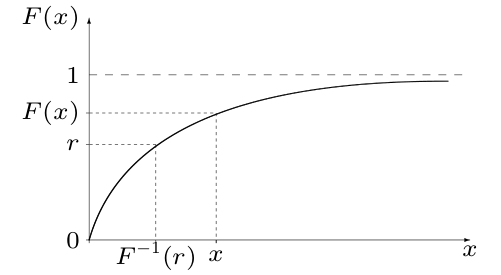
\includegraphics[width=0.65\textwidth]{images/cap11fig1.png}
  \caption{Funzione di distribuzione cumulativa}
  \label{cap11fig1}
\end{figure}

segue inoltre che:

\begin{center}
$F(x) = P(r \leq F(x)) = P(F^{-1}(r) \leq x)$  
\end{center}

cio\`e la funzione $F^{-1}(r)$ ha distribuzione cumulativa data da
$F(x)$ e quindi la sua densit\`a di probabilit\`a \`e
$f(x)$. $\blacksquare$

\par\bigskip

\subsection{Distribuzione uniforme}

Supponiamo di voler generare dei numeri casuali assumendo che abbiano
distribuzione uniforme fra {\em a} e {\em b}. In questi casi la {\bf
  funzione densit\`a di probabilit\`a} \`e:

\begin{center}
$f(x) = \frac{1}{b-a} \quad (a \leq x \leq b)$  
\end{center}

Segue che la {\bf funzione distribuzione cumulativa} \`e:

\begin{center}
$F(x) = \int\limits_{a}^x \frac{1}{b-a}d\xi = \frac{1}{b-a}[\xi]_a^x =
\frac{x-a}{b-a}$
\end{center}

A titolo di esercizio mostriamo anche il calcolo della {\bf speranza}
di tale distribuzione di probabilit\`a \`e:

\begin{center}
$\mathbb{E} = \int\limits_{a}^b\frac{x}{b-a}dx = \frac{1}{b-a}\bigr
  [\frac{x^2}{2} \bigr ]_a^b = \frac{1}{b-a}\cdot\frac{b^2-a^2}{2} =
  \frac{a+b}{2} $
\end{center}

Per generare un numero casuale poniamo $r = \frac{x-a}{b-a}$ ed
otteniamo $x = a + r (b-a)$.

\subsection{Distribuzione esponenziale}

La distribuzione esponenziale di parametro $\lambda$ ha {\bf funzione
densit\`a di probabilit\`a} data da:

\begin{center}
$f(x) = \lambda \cdot e^{-\lambda x} \quad (\lambda > 0, x> 0)$
\end{center}

Da cui segue che che la {\bf funzione di distribuzione cumulativa}
\`e:

\begin{center}
$F(x) = \int\limits_{0}^{x} \lambda \cdot e^{-\lambda \xi} d\xi =
  \lambda \bigr [ - \frac{e^{-\lambda x}}{\lambda} \bigr ]_0^x = 1 -
  e^{-\lambda x}$  
\end{center}

La {\bf funzione valor medio} \`e invece:

\begin{center}
$\mathbb{E}(x) = \frac{1}{\lambda}$  
\end{center}

Per generare un numero casuale poniamo $r = 1-e^{-\lambda x}$ e con
dei semplici passaggi otteniamo $x = -\frac{1}{\lambda} \ln{(1-r)}$.

\end{document}
